\documentclass[aspectratio=169,10pt]{beamer}

% ============================================================
% PACKAGES
% ============================================================
\usetheme{metropolis}
\usepackage{tikz}
\usepackage{amsmath}
\usetikzlibrary{calc,arrows.meta,angles,quotes}

\setbeamertemplate{navigation symbols}{}

% ============================================================
% FOOTER
% ============================================================
\setbeamercolor{footline}{fg=white,bg=mDarkTeal}
\setbeamertemplate{footline}{%
\begin{beamercolorbox}[wd=\paperwidth,ht=3.2ex,dp=1.2ex]{footline}
\hspace{1.2em}\scriptsize Gajavada Sanjeevkumar\hfill
\scriptsize Engineering Curves: Epicycloid\hfill
\scriptsize
\Acrobatmenu{FirstPage}{\fbox{\(\blacktriangleleft\!\blacktriangleleft\)}}\,%
\Acrobatmenu{PrevPage}{\fbox{\(\blacktriangleleft\)}}\,%
\Acrobatmenu{NextPage}{\fbox{\(\blacktriangleright\)}}\,%
\Acrobatmenu{LastPage}{\fbox{\(\blacktriangleright\!\blacktriangleright\)}}\quad
\insertframenumber\hspace{1.2em}
\end{beamercolorbox}}

% ============================================================
% TITLE
% ============================================================
\title[Engineering Curves: Hypocycloid]
{Engineering Curves: Construction of Hypocycloid}
\subtitle{Rolling Circle Method with Tangent \& Normal}
\author{Gajavada Sanjeevkumar}
\date{\today}

% ============================================================
% TIKZ STYLES
% ============================================================
\tikzset{
    extension line/.style={thin, densely dotted, violet!70},
    directing line/.style={thick, blue!80!black},
    generating line/.style={thick, green!60!black},
    centre line/.style={
        thin,
        dash pattern=on 8pt off 2pt on 1.5pt off 2pt,
        red!70!black
    },
    construction line/.style={thin, cyan!80!black},
    division line/.style={thin, orange!90!black},
    arc line/.style={thin, purple!80!black},
    main curve/.style={thick, blue!90!black},
    normal line/.style={thick, orange!90!black},
    tangent line/.style={thick, magenta!90!black},
    contact line/.style={thin, brown!70!black},
    dimension line/.style={thin, <->, >=Stealth, black!75}
}

% ============================================================
% CONSTANTS
% ============================================================
\def\R{85}
\def\r{25}
\def\Rc{60}
\def\Aang{135}
\def\Bang{29.11764706}
\def\dang{8.823529412}
\def\rollratio{2.4}
\def\thetamax{105.88235294}

% ============================================================
% LEGEND
% ============================================================
\newcommand{\Legend}[1]{%
\node[
    draw=gray!35,
    fill=white,
    rounded corners=2pt,
    inner sep=3pt,
    anchor=north east,
    align=left,
    font=\scriptsize,
    text width=31mm
] at (110.67,84){#1};
}

% ============================================================
% BASIC GEOMETRY
% ============================================================
\newcommand{\Base}{%
    \coordinate(O) at (0,0);
    \coordinate(A) at (\Aang:\R);
    \coordinate(B) at (\Bang:\R);
    \coordinate(Czero) at (\Aang:\Rc);

    \draw[thin] (O)--(A);
    \draw[thin] (O)--(B);
    \draw[extension line] (A)--(\Aang:98);
    \draw[extension line] (B)--(\Bang:98);
    \draw[directing line] (A) arc (\Aang:\Bang:\R);

    \fill(O) circle (.7pt) node[below] {$O$};
    \fill(A) circle (.6pt) node[above left] {$A$};
    \fill(B) circle (.6pt) node[below right] {$B$};
}

% ============================================================
% DIMENSIONING
% ============================================================
\newcommand{\OADim}{%
    \draw[dimension line]
        ($(O)+(225:9)$)--($(A)+(225:9)$)
        node[midway,sloped,below,fill=white,inner sep=1pt,
        font=\scriptsize] {$85\ \mathrm{mm}$};
    \draw[thin,black!55] (O)--($(O)+(225:9)$);
    \draw[thin,black!55] (A)--($(A)+(225:9)$);
}

\newcommand{\ACDim}{%
    \draw[dimension line]
        ($(A)+(225:7)$)--($(Czero)+(225:7)$)
        node[midway,sloped,above,fill=white,inner sep=1pt,
        font=\scriptsize] {$25\ \mathrm{mm}$};
    \draw[thin,black!55] (A)--($(A)+(225:7)$);
    \draw[thin,black!55] (Czero)--($(Czero)+(225:7)$);
}

\newcommand{\OCDim}{%
    \draw[dimension line]
        ($(O)+(225:12)$)--($(Czero)+(225:12)$)
        node[midway,sloped,below,fill=white,inner sep=1pt,
        font=\scriptsize] {$60\ \mathrm{mm}$};
    \draw[thin,black!55] (O)--($(O)+(225:12)$);
    \draw[thin,black!55] (Czero)--($(Czero)+(225:12)$);
}

% ============================================================
% INITIAL GENERATING CIRCLE
% ============================================================
\newcommand{\DrawCzero}{%
    \draw[centre line] (O)--(Czero);
    \fill[black] (Czero) circle (1.6pt) node[above left,font=\scriptsize,black,xshift=-2pt,yshift=2pt] {$C_0$};
}

\newcommand{\GenCircle}{%
    \draw[generating line] (Czero) circle (\r);
}

\newcommand{\GenPt}[1]{%
    \coordinate(G#1) at ($(Czero)+({\Aang-30*(#1)}:\r)$);
    \fill[black] (G#1) circle (.45pt);
}

\newcommand{\GenRad}[1]{%
    \draw[construction line] (Czero)--(G#1);
}

\newcommand{\GenLab}[1]{%
    \node[font=\tiny,green!50!black]
    at ($(Czero)+({\Aang-30*(#1)}:28.5)$) {$#1$};
}

\newcommand{\AllGen}{%
    \foreach\k in {0,...,12}{\GenPt{\k}}
}
\newcommand{\AllGenRad}{%
    \foreach\k in {0,...,11}{\GenRad{\k}}
}
\newcommand{\AllGenLab}{%
    % G_0 and G_12 coincide: show the label only once.
    \node[font=\tiny,green!50!black,above left,inner sep=.5pt]
    at ($(G0)+(135:5)$) {$0,\ 12$};
    \foreach\k in {1,...,11}{\GenLab{\k}}
}

% ============================================================
% HYPOCYCLOID COORDINATES
% ============================================================
\newcommand{\AllPCoords}{%
    \foreach\k in {0,...,12}{%
        \coordinate(P\k) at (
            {60*cos(135-\dang*(\k))
             +25*cos(135+\rollratio*\dang*(\k))},
            {60*sin(135-\dang*(\k))
             +25*sin(135+\rollratio*\dang*(\k))}
        );
    }%
}

% ============================================================
% CONCENTRIC CONSTRUCTION ARCS
% ============================================================
% The initial generating-circle divisions are clockwise:
% G_k = C_0 + r at angle (A - 30 k).
% With O as centre, draw concentric arcs through these points.
% |OG_k| = |OG_(12-k)|, so each pair shares one physical arc.

\newcommand{\ConArcPair}[2]{%
    \pgfmathsetmacro{\gx}{
        60*cos(135)+25*cos(135-30*(#1))
    }
    \pgfmathsetmacro{\gy}{
        60*sin(135)+25*sin(135-30*(#1))
    }
    \pgfmathsetmacro{\rr}{sqrt(\gx*\gx+\gy*\gy)}
    \pgfmathsetmacro{\aa}{atan2(\gy,\gx)}
    \draw[arc line]
        (\aa:\rr) arc (\aa:\Bang:\rr);
}

\newcommand{\ConArcZero}{%
    \draw[arc line]
        (\Aang:\R) arc (\Aang:\Bang:\R);
}

\newcommand{\ConFull}{%
    \ConArcZero
    \ConArcPair{11}{11}
    \ConArcPair{10}{10}
    \ConArcPair{9}{9}
    \ConArcPair{8}{8}
    \ConArcPair{7}{7}
    \ConArcPair{6}{6}
}

% ============================================================
% CENTRE LOCUS
% ============================================================
\newcommand{\CentreArc}{%
    \draw[centre line]
        (\Aang:\Rc) arc (\Aang:\Bang:\Rc);
}

% ============================================================
% ANGULAR DIVISIONS
% ============================================================
\newcommand{\DivLine}[1]{%
    \draw[division line]
        (O)--({135-\dang*(#1)}:\R);
}

\newcommand{\DivLabel}[1]{%
    \node[
        font=\tiny,
        orange!90!black,
        inner sep=.5pt
    ] at ({135-\dang*(#1)}:91) {$#1^\prime$};
}

\newcommand{\CenterPt}[1]{%
    \coordinate(C#1) at ({135-\dang*(#1)}:\Rc);
    \node[circle,fill=black,inner sep=0pt,minimum size=4.5pt] at(C#1) {};
    \node[font=\scriptsize,above right,inner sep=1.2pt,text=black]
        at(C#1) {$C_{#1}$};
}

\newcommand{\AllDiv}{%
    \foreach\k in {0,...,12}{\DivLine{\k}}
}
\newcommand{\AllLabels}{%
    \foreach\k in {0,...,12}{\DivLabel{\k}}
}
\newcommand{\AllCenters}{%
    \foreach\k in {0,...,12}{\CenterPt{\k}}
}
\newcommand{\DivFull}{%
    \AllDiv\AllLabels\AllCenters
}

% ============================================================
% CUTTING ARCS
% ============================================================
\newcommand{\CutArc}[1]{%
    \pgfmathsetmacro{\qa}{135+\rollratio*\dang*(#1)}
    \draw[construction line,very thin]
        (C#1)+({\qa-12}:25)
        arc({\qa-12}:{\qa+12}:25);
}

\newcommand{\Pmark}[1]{%
    \node[circle,fill=black,inner sep=0pt,minimum size=4.5pt] at(P#1) {};
    \ifnum#1>0
        \node[
            font=\scriptsize,
            black,
            above right,
            xshift=2pt,
            yshift=2pt,
            inner sep=1pt
        ] at(P#1) {$P_{#1}$};
    \fi
}

\newcommand{\AllCut}{%
    \AllPCoords
    \foreach\k in {1,...,12}{%
        \CutArc{\k}\Pmark{\k}
    }%
}

% ============================================================
% HYPOCYCLOID
% ============================================================
\newcommand{\Curve}{%
    \draw[main curve]
    plot[
        domain=0:\thetamax,
        samples=360,
        variable=\th,
        smooth
    ] (
        {60*cos(135-\th)+25*cos(135+\rollratio*\th)},
        {60*sin(135-\th)+25*sin(135+\rollratio*\th)}
    );
}

% ============================================================
% SELECTED POINT & GEOMETRY (Dynamically Derived Normal & Tangent)
% ============================================================
\newcommand{\SelectedGeometry}{%
    % Right-side OP=50 mm intersection of the hypocycloid.
    % theta_P = 69.08834347 deg.
    \coordinate(Psel) at (37.29426240,33.30372340);

    % Corresponding generating-circle centre:
    % angle C_p O = 135 - theta_P = 65.91165653 deg.
    \coordinate(Cp) at (65.91165653:60);

    % M is where OC_p meets the directing arc AB.
    \coordinate(M) at (65.91165653:85);

    % PM is the normal.
    \def\NormAng{93.36184043}
    \coordinate(NNright) at ($(Psel)+(\NormAng:48)$);
    \coordinate(NNleft)  at ($(Psel)+(\NormAng+180:30)$);

    % Tangent perpendicular to PM.
    \coordinate(T1) at ($(Psel)+(183.36184043:48)$);
    \coordinate(T2) at ($(Psel)+(3.36184043:48)$);
}

\newcommand{\PGeometry}{%
    \node[circle,fill=black,inner sep=0pt,minimum size=5pt] at(Psel) {};
    \node[
        font=\scriptsize,
        black,
        above right,
        xshift=3pt,
        yshift=3pt,
        inner sep=1pt
    ] at(Psel) {$P$};
}

\newcommand{\PtoCpArc}{%
    % PC_p = 25 mm.
    % Direction P -> C_p = 120.81202433 deg.
    \draw[construction line,very thin]
        (Psel)+(108.81202433:25)
        arc(108.81202433:132.81202433:25);

    \draw[construction line] (Psel)--(Cp);

    \node[circle,fill=black,inner sep=0pt,minimum size=4.5pt] at(Cp) {};
    \node[
        font=\scriptsize,
        black,
        above right,
        xshift=3pt,
        yshift=3pt,
        inner sep=1pt
    ] at(Cp) {$C_p$};

    % Dimension line parallel to PC_p.
    % Limiting lines are perpendicular to PC_p.
    \draw[dimension line]
        ($(Psel)+(30.81202433:6)$)--($(Cp)+(30.81202433:6)$)
        node[
            midway,
            sloped,
            above,
            fill=white,
            inner sep=1pt,
            font=\scriptsize
        ] {$25\ \mathrm{mm}$};

    \draw[thin,black!55]
        (Psel)--($(Psel)+(30.81202433:6)$);
    \draw[thin,black!55]
        (Cp)--($(Cp)+(30.81202433:6)$);
}

% ============================================================
% NORMAL AND TANGENT
% ============================================================
\newcommand{\NormalLine}{%
    \draw[normal line,line width=1.2pt]
        (NNleft)--(NNright);

    \node[
        font=\scriptsize,
        orange!85!black,
        above right,
        xshift=2pt
    ] at(NNright) {$N'$};

    \node[
        font=\scriptsize,
        orange!85!black,
        below left,
        xshift=-2pt
    ] at(NNleft) {$N$};
}

\newcommand{\NormalAndTangent}{%
    \NormalLine

    \draw[tangent line,line width=1.2pt]
        (T2)--(T1);

    \node[
        font=\scriptsize,
        magenta!80!black,
        above right,
        xshift=2pt
    ] at(T1) {$T'$};

    \node[
        font=\scriptsize,
        magenta!80!black,
        below left,
        xshift=-2pt
    ] at(T2) {$T$};
}

% ============================================================
% CONSTRUCTION BUNDLES
% ============================================================
\newcommand{\BaseCommon}{%
    \Base\DrawCzero\GenCircle
}

\newcommand{\GenFull}{%
    \AllGen\AllGenRad\AllGenLab
}

\newcommand{\FinalConstruction}{%
    \BaseCommon
    \GenFull
    \ConFull
    \CentreArc
    \DivFull
    \AllCut
    \Curve
}

% ============================================================
% DOCUMENT
% ============================================================
\begin{document}

\begin{frame}[plain]
    \titlepage
\end{frame}

\begin{frame}{Problem Statement}
\begin{block}{Problem}

Draw a hypocycloid of a circle of diameter 50 mm, which rolls inside a circular arc of radius 85 mm for one revolution. Also, draw a tangent and a normal to the epicycloid at a point 50 mm from the centre of the directing circle.
\end{block}
\end{frame}

\begin{frame}{Calculated Data}
\begin{align*}
R &= 85\text{ mm},
&
r &= \frac{50}{2}=25\text{ mm},
\\[0.4em]
OC_0 &= R-r=85-25=60\text{ mm},
&
AC_0 &=25\text{ mm},
\\[0.4em]
\angle AOB
&=360^\circ\frac{r}{R}
=360^\circ\frac{25}{85}
=105.882353^\circ,
\\[0.4em]
\Delta\theta
&=\frac{105.882353^\circ}{12}
=8.823529^\circ,
&
\text{Generating-circle division}
&=30^\circ.
\end{align*}
\end{frame}



\begin{frame}{Step 1: Draw $OA$}
\centering
\begin{tikzpicture}[scale=.075,>=stealth,rotate=0]
    \coordinate(O)at(0,0);
    \coordinate(A)at(135:85);
    \draw[thin](O)--(A);
    \draw[dimension line]
        ($(O)+(225:9)$)--($(A)+(225:9)$)
        node[midway,sloped,below,fill=white,inner sep=1pt,
        font=\scriptsize]{$85\ \mathrm{mm}$};
    \draw[thin,black!55](O)--($(O)+(225:9)$);
    \draw[thin,black!55](A)--($(A)+(225:9)$);
    \fill(O)circle(.7pt)node[below]{$O$};
    \fill(A)circle(.6pt)node[above left]{$A$};
    \Legend{$OA=85$ mm.}
\end{tikzpicture}
\end{frame}


\begin{frame}{Step 2: Draw $OB$ at $105.88^\circ$}
\centering
\begin{tikzpicture}[scale=.075,>=stealth,rotate=0]
    \coordinate(O)at(0,0);
    \coordinate(A)at(135:85);
    \coordinate(B)at(29.11764706:85);

    \draw[thin](O)--(A);
    \draw[extension line](A)--(135:98);
    \draw[thin](O)--(B);

    \draw[thin,black!70]
        (135:18) arc(135:29.11764706:18);
    \node[font=\scriptsize]at(82:23){$105.88^\circ$};

    \fill(O)circle(.7pt)node[below]{$O$};
    \fill(A)circle(.6pt)node[above left]{$A$};
    \fill(B)circle(.6pt)node[below right]{$B$};

    \Legend{$\angle AOB=105.88^\circ$.}
\end{tikzpicture}
\end{frame}


\begin{frame}{Step 3: Draw the directing arc $AB$}
\centering
\begin{tikzpicture}[scale=.075,>=stealth,rotate=0]
    \Base
    \Legend{Blue arc $AB$: directing circle.}
\end{tikzpicture}
\end{frame}

\begin{frame}{Step 4: Locate $C_0$ and the generating circle}
\centering
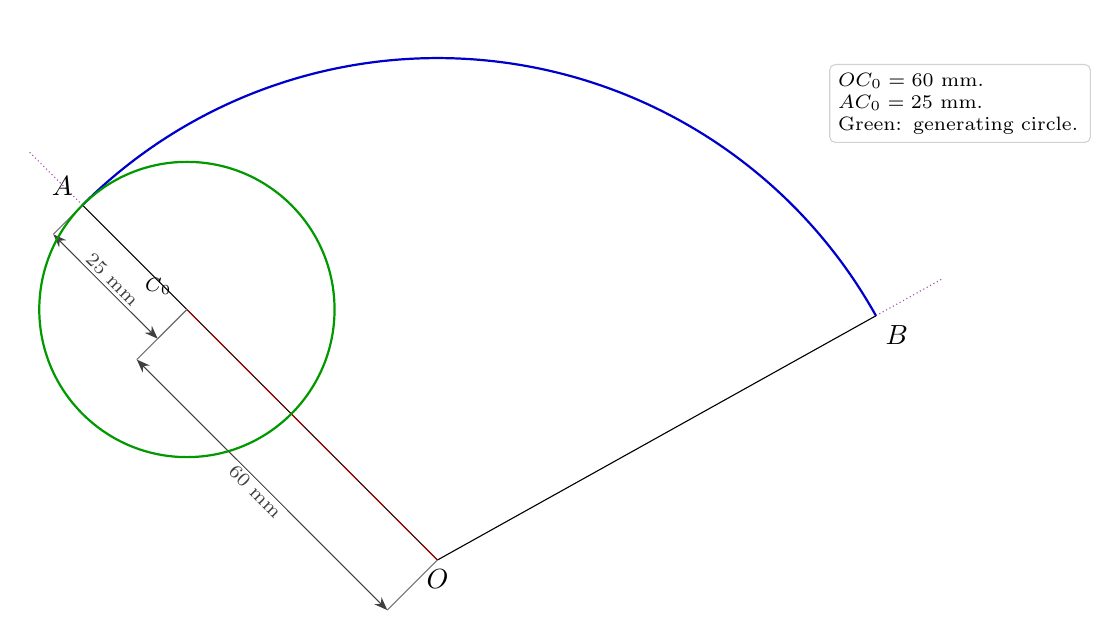
\begin{tikzpicture}[scale=.075,>=stealth,rotate=0]
    \Base
    \DrawCzero
    \ACDim
    \OCDim
    \GenCircle
    \Legend{$OC_0=60$ mm.\\$AC_0=25$ mm.\\Green: generating circle.}
\end{tikzpicture}
\end{frame}

\newcommand{\GenDivisionFrame}[1]{%
\begin{frame}{Step 5: Divide the generating circle into 12 equal parts}
\centering
\begin{tikzpicture}[scale=.075,>=stealth,rotate=0]
    \Base
    \DrawCzero
    \GenCircle

    \foreach\j in {0,...,#1}{%
        \GenPt{\j}%
        \ifnum\j>0
            \GenRad{\j}%
        \fi
    }

    \ifnum#1=12
        % G_0 and G_12 coincide: show the combined label only once.
        \node[
            font=\tiny,
            green!50!black,
            above right,
            inner sep=.5pt
        ] at($(G0)+(135:5)$){$0,\,12$};
    \else
        \node[
            font=\tiny,
            green!50!black,
            below left,
            inner sep=.5pt
        ] at($(G0)+(135:5)$){$0$};
    \fi

    \ifnum#1>0
        \foreach\j in {1,...,#1}{\GenLab{\j}}
    \fi

    \Legend{Green: generating circle.\\Clockwise $30^\circ$ divisions.}
\end{tikzpicture}
\end{frame}
}

\GenDivisionFrame{1}
\GenDivisionFrame{2}
\GenDivisionFrame{3}
\GenDivisionFrame{4}
\GenDivisionFrame{5}
\GenDivisionFrame{6}
\GenDivisionFrame{7}
\GenDivisionFrame{8}
\GenDivisionFrame{9}
\GenDivisionFrame{10}
\GenDivisionFrame{11}
\GenDivisionFrame{12}

\begin{frame}{Step 6: Complete the generating-circle divisions}
\centering
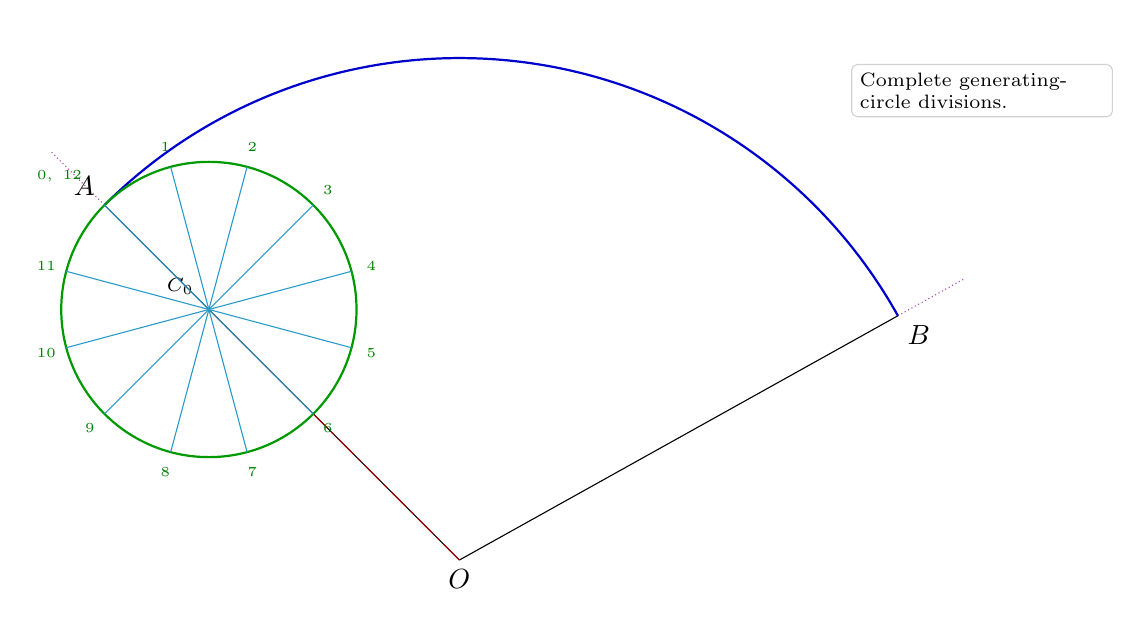
\begin{tikzpicture}[scale=.075,>=stealth,rotate=0]
    \Base
    \DrawCzero
    \GenCircle
    \GenFull
    \Legend{Complete generating-circle divisions.}
\end{tikzpicture}
\end{frame}

\newcommand{\ConFrame}[1]{%
\begin{frame}{Step 7: Draw concentric construction arcs}
\centering
\begin{tikzpicture}[scale=.075,>=stealth,rotate=0]
    \Base
    \DrawCzero
    \GenCircle
    \GenFull
    #1
    \Legend{Construction arcs centered at $O$.\\Equal-radius pairs are used.}
\end{tikzpicture}
\end{frame}
}

\ConFrame{\ConArcZero}
\ConFrame{\ConArcZero\ConArcPair{11}{11}}
\ConFrame{\ConArcZero\ConArcPair{11}{11}\ConArcPair{10}{10}}
\ConFrame{\ConArcZero\ConArcPair{11}{11}\ConArcPair{10}{10}\ConArcPair{9}{9}}
\ConFrame{\ConArcZero\ConArcPair{11}{11}\ConArcPair{10}{10}\ConArcPair{9}{9}\ConArcPair{8}{8}}
\ConFrame{\ConArcZero\ConArcPair{11}{11}\ConArcPair{10}{10}\ConArcPair{9}{9}\ConArcPair{8}{8}\ConArcPair{7}{7}}
\ConFrame{\ConArcZero\ConArcPair{11}{11}\ConArcPair{10}{10}\ConArcPair{9}{9}\ConArcPair{8}{8}\ConArcPair{7}{7}\ConArcPair{6}{6}}

\begin{frame}{Step 8: Draw the centre arc through $C_0$}
\centering
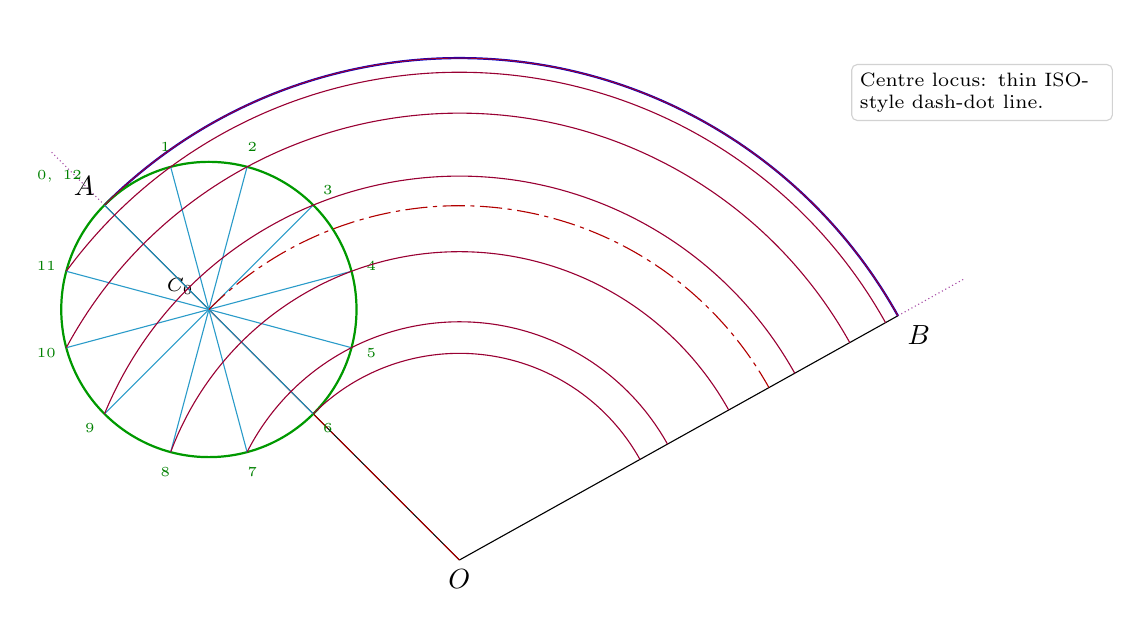
\begin{tikzpicture}[scale=.075,>=stealth,rotate=0]
    \Base
    \DrawCzero
    \GenCircle
    \GenFull
    \ConFull
    \CentreArc
    \Legend{Centre locus: thin ISO-style dash-dot line.}
\end{tikzpicture}
\end{frame}

\newcommand{\AngleFrame}[1]{%
\begin{frame}{Step 9: Divide $\angle AOB$ into 12 equal parts}
\centering
\begin{tikzpicture}[scale=.075,>=stealth,rotate=0]
    \Base
    \DrawCzero
    \GenCircle
    \GenFull
    \ConFull
    \CentreArc

    \foreach\j in {0,...,#1}{%
        \DivLine{\j}
        \DivLabel{\j}
        \CenterPt{\j}
    }

    \Legend{$8.823529^\circ$ divisions.}
\end{tikzpicture}
\end{frame}
}

\AngleFrame{0}
\AngleFrame{1}
\AngleFrame{2}
\AngleFrame{3}
\AngleFrame{4}
\AngleFrame{5}
\AngleFrame{6}
\AngleFrame{7}
\AngleFrame{8}
\AngleFrame{9}
\AngleFrame{10}
\AngleFrame{11}
\AngleFrame{12}

\begin{frame}{Step 10: Complete the angular divisions and centre points}
\centering
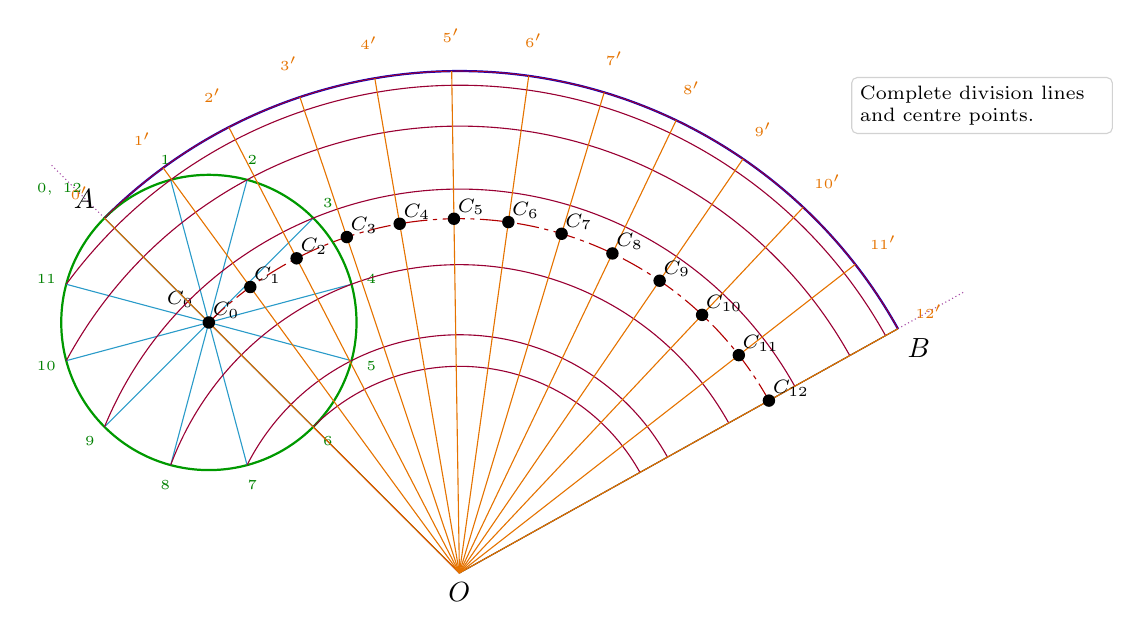
\begin{tikzpicture}[scale=.075,>=stealth,rotate=0]
    \Base
    \DrawCzero
    \GenCircle
    \GenFull
    \ConFull
    \CentreArc
    \DivFull
    \Legend{Complete division lines and centre points.}
\end{tikzpicture}
\end{frame}

\newcommand{\CutFrame}[1]{%
\begin{frame}{Step 11: Draw the cutting arc and locate $P_i$}
\centering
\begin{tikzpicture}[scale=.075,>=stealth,rotate=0]
    \Base
    \DrawCzero
    \GenCircle
    \GenFull
    \ConFull
    \CentreArc
    \DivFull
    \AllPCoords

    \ifnum#1>0
        \foreach\j in {1,...,#1}{%
            \CutArc{\j}
            \Pmark{\j}
        }
    \fi

    \Legend{Cyan cutting arc: radius $25$ mm.}
\end{tikzpicture}
\end{frame}
}

\CutFrame{0}
\CutFrame{1}
\CutFrame{2}
\CutFrame{3}
\CutFrame{4}
\CutFrame{5}
\CutFrame{6}
\CutFrame{7}
\CutFrame{8}
\CutFrame{9}
\CutFrame{10}
\CutFrame{11}
\CutFrame{12}

\begin{frame}{Step 12: Draw the hypocycloid}
\centering
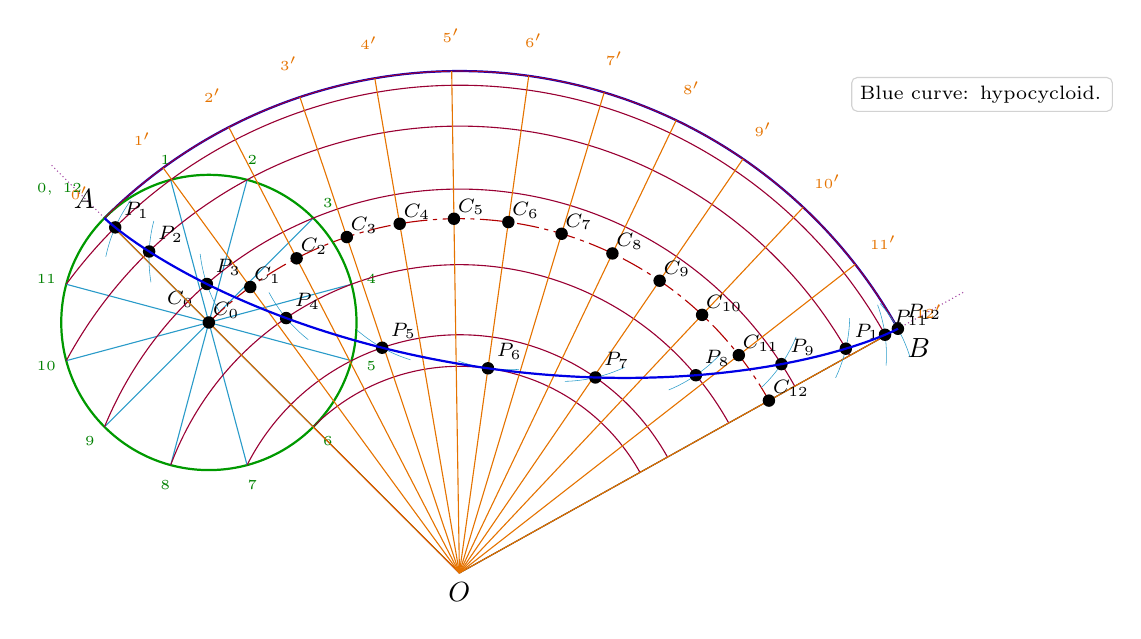
\begin{tikzpicture}[scale=.075,>=stealth,rotate=0]
    \FinalConstruction
    \Legend{Blue curve: hypocycloid.}
\end{tikzpicture}
\end{frame}

\begin{frame}{Step 13: Locate $P$ at $50$ mm from $O$}
\centering
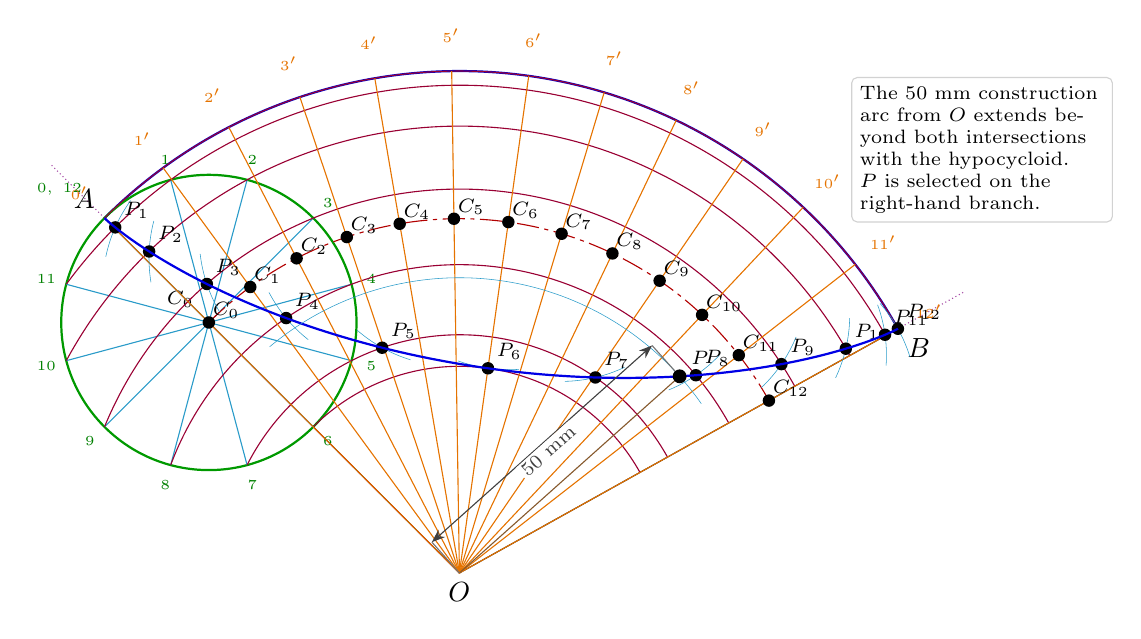
\begin{tikzpicture}[scale=.075,>=stealth,rotate=0]
    \FinalConstruction
    \SelectedGeometry

    % 50-mm construction arc from O, extended to meet the hypocycloid on both sides.
    \draw[construction line,very thin]
        (35:50)
        arc(35:130:50);

    % Radius from O to the selected right-side point P.
    \draw[contact line] (O)--(Psel);

    % Dimension line parallel to OP.
    \draw[dimension line]
        ($(O)+(131.76480853:7)$)--($(Psel)+(131.76480853:7)$)
        node[
            midway,
            sloped,
            below,
            fill=white,
            inner sep=1pt,
            font=\scriptsize
        ] {$50\ \mathrm{mm}$};

    \draw[thin,black!55]
        (O)--($(O)+(131.76480853:7)$);
    \draw[thin,black!55]
        (Psel)--($(Psel)+(131.76480853:7)$);

    \PGeometry
    \Legend{The $50$ mm construction arc from $O$ extends beyond both intersections with the hypocycloid.\\
    $P$ is selected on the right-hand branch.}
\end{tikzpicture}
\end{frame}

\begin{frame}{Step 14: Draw the $25$ mm radius to $C_p$}
\centering
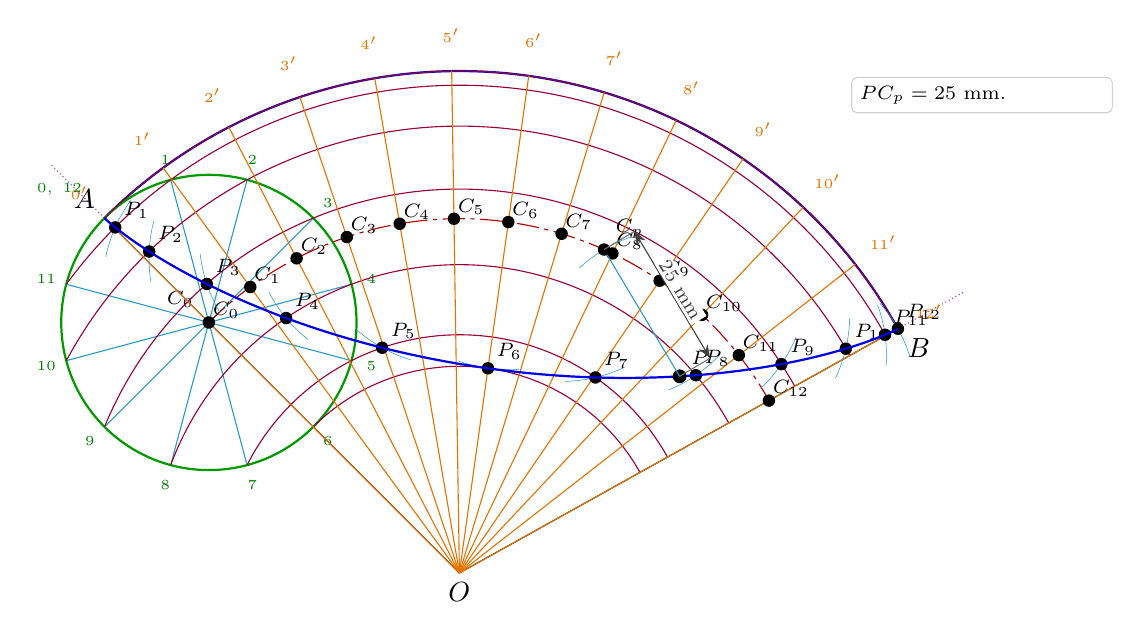
\begin{tikzpicture}[scale=.075,>=stealth,rotate=0]
    \FinalConstruction
    \SelectedGeometry
    \PGeometry
    \PtoCpArc
    \Legend{$PC_p=25$ mm.}
\end{tikzpicture}
\end{frame}

\begin{frame}{Step 15: Extend $OC_p$ to the directing arc $AB$ and mark the intersection $M$}
\centering
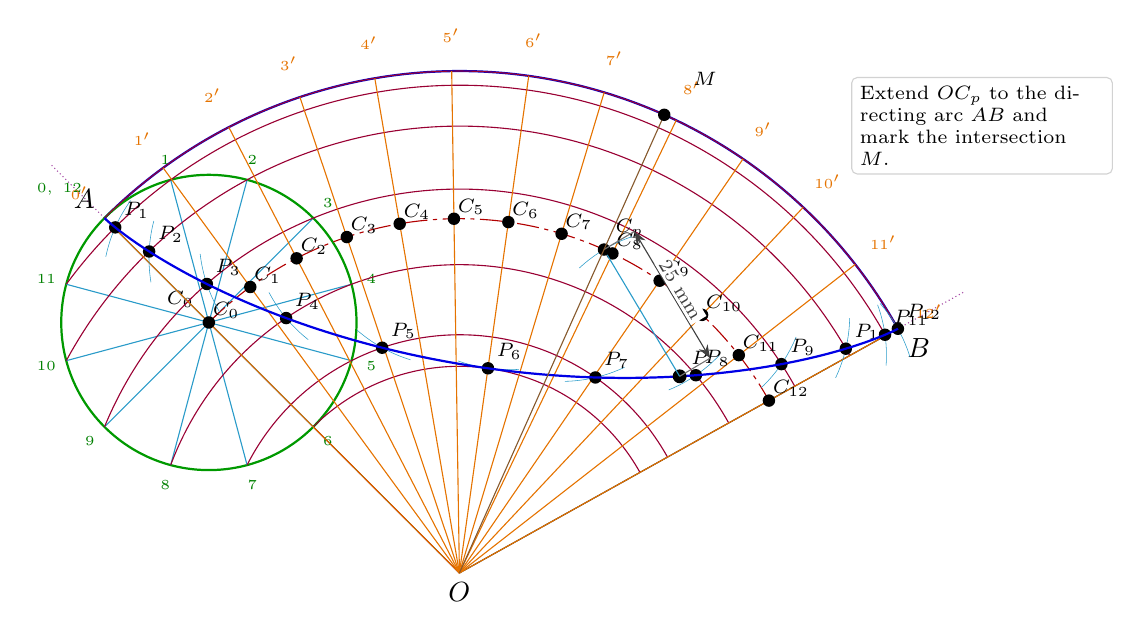
\begin{tikzpicture}[scale=.075,>=stealth,rotate=0]
    \FinalConstruction
    \SelectedGeometry
    \PGeometry
    \PtoCpArc
    \draw[contact line] (O)--(M);
    \node[circle,fill=black,inner sep=0pt,minimum size=4.5pt] at(M) {};
    \node[font=\scriptsize,black,above right,xshift=7pt,yshift=7pt] at(M) {$M$};
    \Legend{Extend $OC_p$ to the directing arc $AB$ and mark the intersection $M$.}
\end{tikzpicture}
\end{frame}

\begin{frame}{Step 16: Mark $M$ on the directing circle}
\centering
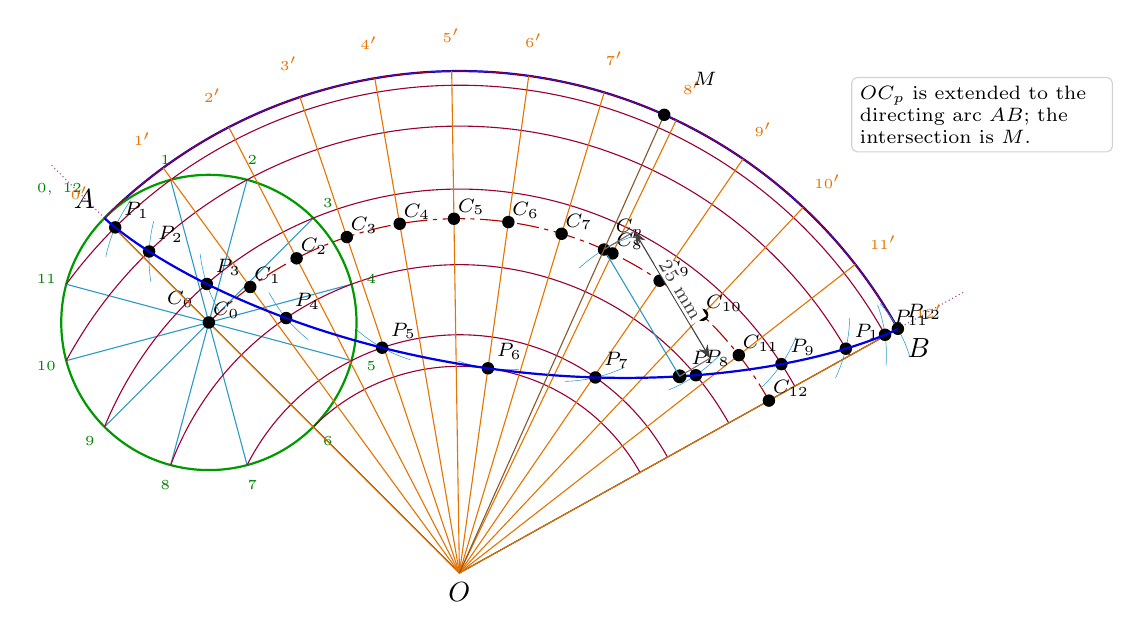
\begin{tikzpicture}[scale=.075,>=stealth,rotate=0]
    \FinalConstruction
    \SelectedGeometry
    \PGeometry
    \PtoCpArc
    \draw[contact line] (O)--(M);

    \node[circle,fill=black,inner sep=0pt,minimum size=4.5pt] at(M) {};
    \node[font=\scriptsize,black,above right,xshift=7pt,yshift=7pt] at(M) {$M$};

    \Legend{$OC_p$ is extended to the directing arc $AB$; the intersection is $M$.}
\end{tikzpicture}
\end{frame}

\begin{frame}{Step 17: Draw the normal $NN'$ through $P$}
\centering
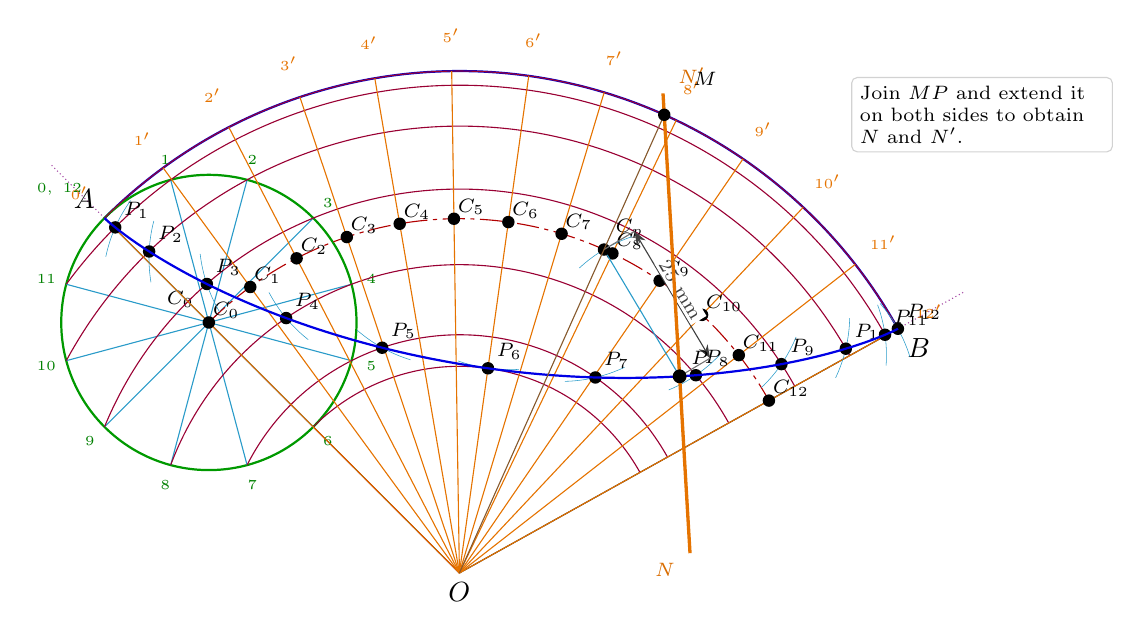
\begin{tikzpicture}[scale=.075,>=stealth,rotate=0]
    \FinalConstruction
    \SelectedGeometry
    \PtoCpArc
    \draw[contact line] (O)--(M);
    \NormalLine
    \PGeometry

    \node[circle,fill=black,inner sep=0pt,minimum size=4.5pt] at(M) {};
    \node[font=\scriptsize,black,above right,xshift=7pt,yshift=7pt] at(M) {$M$};

    \Legend{Join $MP$ and extend it on both sides to obtain $N$ and $N'$.}
\end{tikzpicture}
\end{frame}

\begin{frame}{Step 18: Draw the tangent $TT'$ perpendicular to $NN'$}
\centering
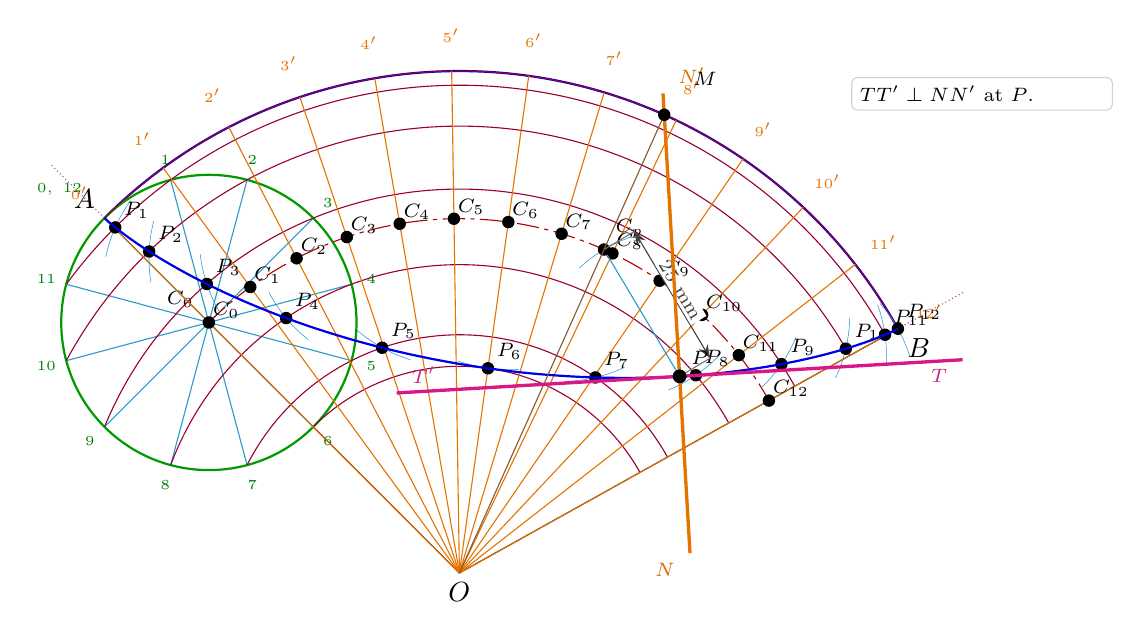
\begin{tikzpicture}[scale=.075,>=stealth,rotate=0]
    \FinalConstruction
    \SelectedGeometry
    \PtoCpArc
    \draw[contact line] (O)--(M);
    \NormalAndTangent
    \PGeometry

    \node[circle,fill=black,inner sep=0pt,minimum size=4.5pt] at(M) {};
    \node[font=\scriptsize,black,above right,xshift=7pt,yshift=7pt] at(M) {$M$};

    \Legend{$TT'\perp NN'$ at $P$.}
\end{tikzpicture}
\end{frame}

\begin{frame}{Step 19: Show the right angle at $P$}
\centering
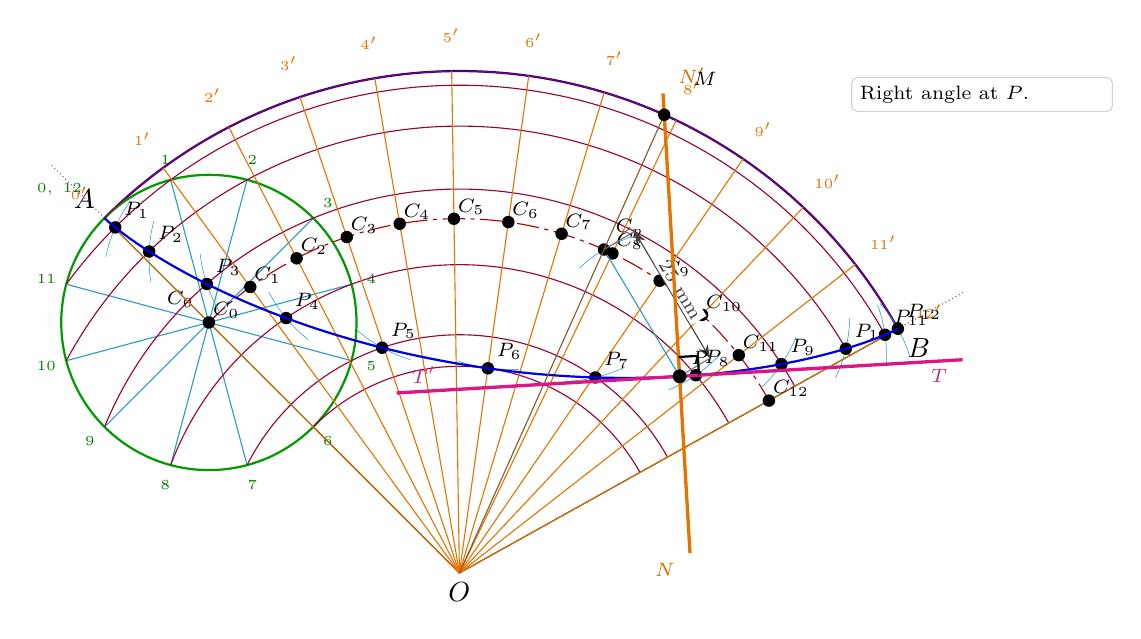
\begin{tikzpicture}[scale=.075,>=stealth,rotate=0]
    \FinalConstruction
    \SelectedGeometry
    \PtoCpArc
    \draw[contact line] (O)--(M);
    \NormalAndTangent
    \PGeometry

    \node[circle,fill=black,inner sep=0pt,minimum size=4.5pt] at(M) {};
    \node[font=\scriptsize,black,above right,xshift=7pt,yshift=7pt] at(M) {$M$};

    \pic[
        draw=black,
        line width=.8pt,
        angle radius=7pt,
        angle eccentricity=1.35
    ] at(Psel) {right angle=T2--Psel--NNright};

    \Legend{Right angle at $P$.}
\end{tikzpicture}
\end{frame}

\begin{frame}{Step 20: Final completed hypocycloid construction}
\centering
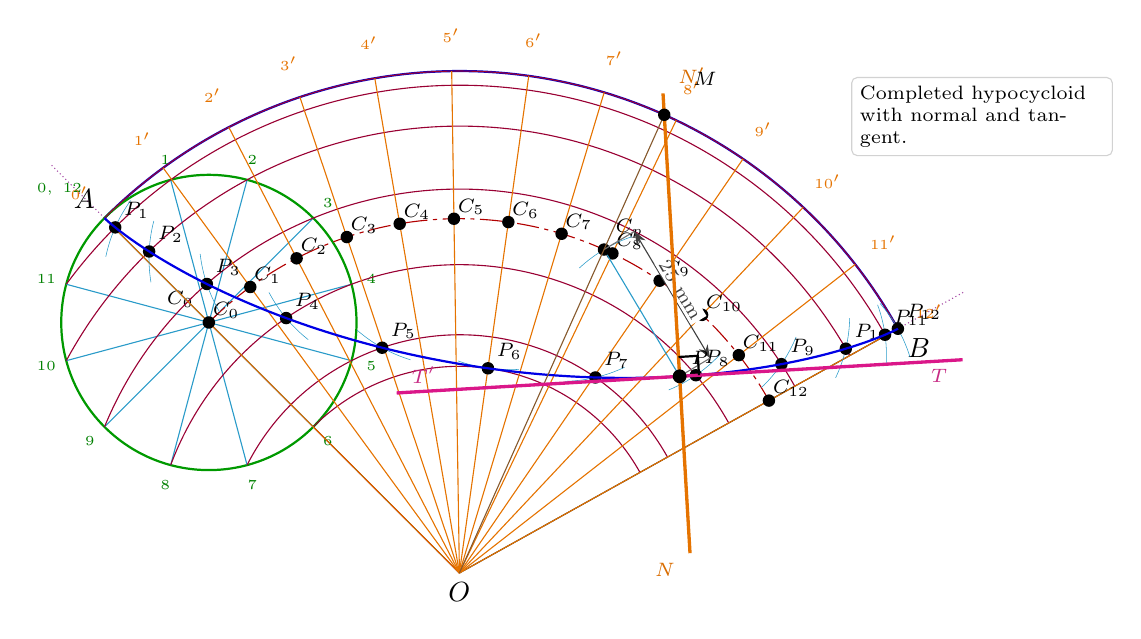
\begin{tikzpicture}[scale=.075,>=stealth,rotate=0]
    \FinalConstruction
    \SelectedGeometry
    \PtoCpArc
    \draw[contact line] (O)--(M);
    \NormalAndTangent
    \PGeometry

    \node[circle,fill=black,inner sep=0pt,minimum size=4.5pt] at(M) {};
    \node[font=\scriptsize,black,above right,xshift=7pt,yshift=7pt] at(M) {$M$};

    \pic[
        draw=black,
        line width=.8pt,
        angle radius=7pt,
        angle eccentricity=1.35
    ] at(Psel) {right angle=T2--Psel--NNright};

    \Legend{Completed hypocycloid with normal and tangent.}
\end{tikzpicture}
\end{frame}

\end{document}